\section{上传与数据集}

不采集也能用。手上有表格时，第一个节点用“\texttt{上传文件}”。

\begin{figure}[H]\centering

\includegraphics[width=0.31\textwidth]{panel-upload.png}
\caption{上传节点：从文件选，或挂一份已存数据集}
\label{fig:panel-upload}
\end{figure}

\subsection{支持的文件}

CSV、TSV、JSON、TXT、Excel 是最常用的五种。文献工具导出的 NBIB、RIS、BibTeX、EndNote、NoteExpress 也能直接读，
程序把它认成文献记录表，不需要先整理列名。

Excel 一次只读一张工作表。一个文件里有好几张非空的表时会拒绝并列出表名，让你先把要的那张单独存出来或转成 CSV。
两张表列不一样，硬合会错位。

\subsection{上传以后发生什么}

文件算一个内容哈希，压进本地库，登记成数据集。以后这份工作流打开时可以直接挂回这份数据，不用再找原文件；
同一份文件重复上传不会存两份，认的是哈希。

“\texttt{数据集}”面板能看到每份文件的来源、列数、行数、被哪些工作流引用，可以改名、删除、合并。
被工作流引用的数据集单独删会当场拒绝，面板顶部的清空是例外，它连被引用的也一起删，确认框里写清了这个区别。

\begin{figure}[H]\centering

\includegraphics[width=0.43\textwidth]{datasets.png}
\caption{数据集面板，一份表格一行}
\label{fig:datasets2}
\end{figure}

上传面板里还有一条捷径，从已保存的数据集里选，适合反复用同一份底表做不同的分析。

\subsection{合并同构的数据集}

两份表列一样时，数据集面板能把它们合并成一份，默认加一列来源记下每一行来自哪份。
列多了少了都会按名字拒绝，并告诉你是哪一列对不上。

\section{清洗}

采集回来的文本很脏：转发链、提及、话题标记、链接、表情代码混在一起，还有水军刷的重复稿。
清洗节点干两件事，剥掉噪音，判断这一行跟主题有没有关系。

“\texttt{正则}”模式不花模型的钱，规则固定。它剥掉转发链只留你自己那段，去掉提及、话题标记、链接与表情代码，
整行只剩这些东西的判为删除。原文保留，清洗结果写在 \texttt{cleaned\_text} 列。
“\texttt{模型}”模式逐行问一次模型，判断内容是否与主题相关，顺便过滤广告与灌水，更聪明也更慢，几千行以上要算清成本。

\section{去重}

去重不是一个算子，是三个，按粗到细排。

\begin{figure}[H]\centering
\begin{tikzpicture}[node distance=6mm]
  \node[card=src,text width=2.5cm] (raw) {原始行\\[2pt]\micro 3000 条};
  \node[card=prc,right=of raw,text width=2.7cm] (exact) {逐字去重\\[2pt]\micro 完全相同才删};
  \node[card=anl,right=of exact,text width=2.7cm] (norm) {归一化去重\\[2pt]\micro 忽略链接与标记};
  \node[card=viz,right=of norm,text width=2.7cm] (sim) {近重复去重\\[2pt]\micro 指纹距离};
  \draw[wire] (raw) -- (exact);
  \draw[wire] (exact) -- (norm);
  \draw[wire] (norm) -- (sim);
  \node[micro,below=5pt of norm] {改写的水军稿在这里被抓到};
  \node[micro,below=5pt of sim] {改一个词的转发在这里被抓到};
\end{tikzpicture}
\caption{三层去重，一层比一层松}
\label{fig:dedupe}
\end{figure}

逐字去重看整行是否完全一样。归一化去重在比较之前先把链接、提及、话题、表情抹平，所以同一句话换个链接发两次也能认出来。
近重复去重用 SimHash 指纹，距离默认八位，抓改了一个词的转发。距离调大召回更高、精确率更低；
微博评论里改一个词大约差五到十八位，两条互不相关的评论差二十六到二十八位，所以八是个合理的起点。

\section{确定性算子}

分析节点里有一批不需要模型的算子，日常清理够用。

\begin{table}[H]\centering
\caption{常用确定性算子}
\label{tab:ops}
\small
\begin{tabularx}{\textwidth}{p{3.2cm}X}
\toprule
算子 & 用途 \\
\midrule
去空值 & 任一列为空即删，或全部为空才删 \\
填充空值 & 填一个值，或者前向、后向填充 \\
条件筛选 & 按一列的值保留行，等于、不等于、包含、为空 \\
选择列 & 只留要的几列，顺序按你写的来 \\
重命名列 & 上游列名不合适时在这里改 \\
去除空白 & 去掉首尾空格，中文全角空格也清 \\
类型转换 & 文本转数字、转日期 \\
排序 & 按一列或多列排，升降序可选 \\
采样 & 随机抽若干行，做小样本试验 \\
分组聚合 & 按一列分组，对另一列求和、均值、计数 \\
表关联 & 两张表按一个键拼起来 \\
列计算 & 两列相加、相除，结果写进新列 \\
数值分箱 & 等宽分箱，或自己给边界与标签 \\
\bottomrule
\end{tabularx}
\end{table}

这些算子出错会直接失败，不给一张空表：给文本列求和、比较条件填了非数字、指定的列不存在，都属于这一类，
报错信息会点名是哪个节点、哪一列。

\section{时间与阶段}

做事件研究要先有阶段。三个算子把时间拆开，各管一段。

“\texttt{提取时间}”从时间列派生新列，可以派生日期、小时、星期、月份。解析不了的相对时间标签留空，程序不猜年份。

“\texttt{按时间划分阶段}”用一串边界给行打阶段标签，规则是左闭右开，边界前一天二十三点五十九分的行还算前一个阶段。
面板里填三样：列选时间列，边界从早到晚写，最后一个边界是最后阶段的次日；阶段名按顺序写，个数比边界少一个。

\begin{figure}[H]\centering
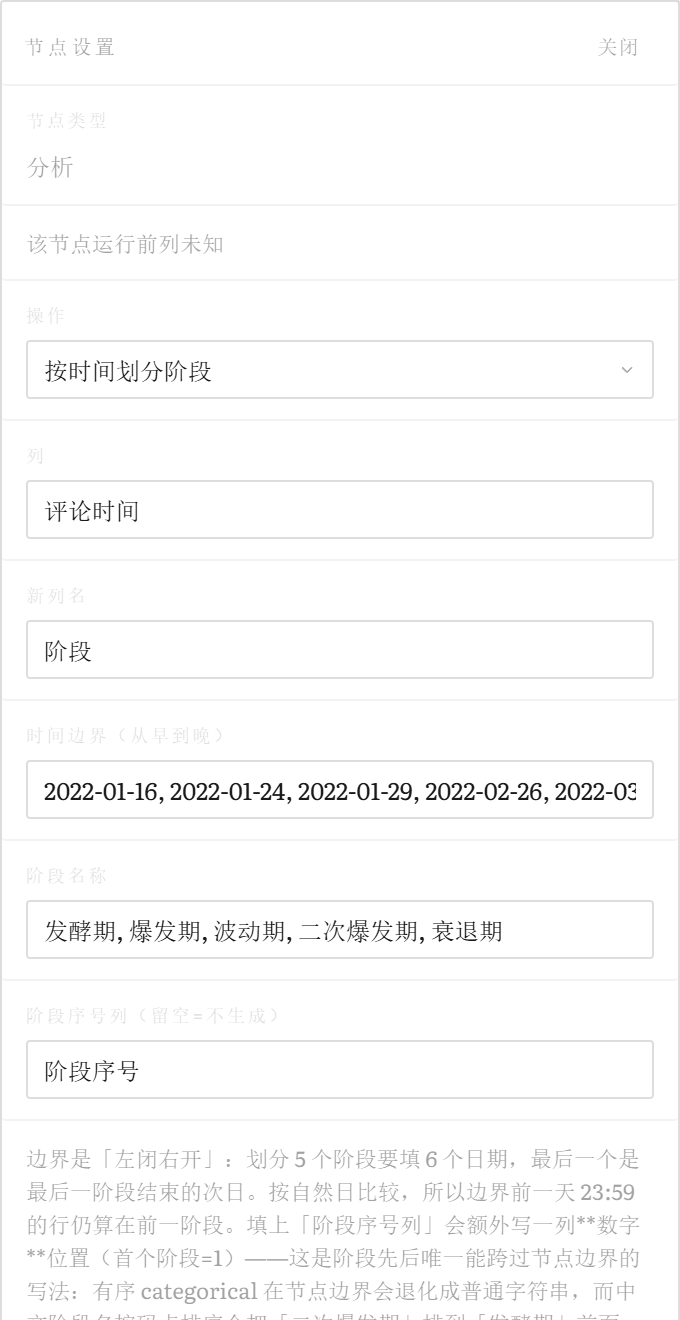
\includegraphics[width=0.31\textwidth]{liu-stage.png}
\caption{划分阶段：六条边界切出五个阶段}
\label{fig:liu-stage}
\end{figure}

“\texttt{阶段序号列}”建议填上。阶段列是有序的类别，但每过一个节点表格会被重建成普通文本，
中文阶段名按字符码排序会把“二次爆发期”排到“发酵期”前面，一张按阶段分组的表就读反了，而它看起来依旧完整。
所以划分阶段会额外写一列数字，第一阶段是一，往后递增。分阶段主题、主题生命周期、主题流向这些要按先后算的步骤读的都是这一列数字，
两个都没有时它们会拒绝，不按名字猜先后。

不知道边界怎么切时，用“\texttt{按发文量建议阶段边界}”。它读每日发文曲线的峰谷，把能直接粘进上一步的边界与标签打印出来。
峰的定义是一段连续若干天高于日常中位数若干倍，太短的窗口会并入行数更多的邻居，并提醒你并了哪一段。
